\documentclass[11pt]{thesistemp}

\usepackage[italian]{babel}
\usepackage[utf8]{inputenc}
\usepackage{adjustbox}
\usepackage{subcaption}
\usepackage{graphicx}
\usepackage{wrapfig}

\graphicspath{ {../media/} }

\usepackage{hyperref}

%----------------------------------------------------------------------------------------
%	TITLE
%----------------------------------------------------------------------------------------

\title{Servizi di supporto alle transazioni su Blockchain Ethereum}
\creationdate{10 Novembre 2018}
\redactedby{Aaron Cesaro}

\begin{document}

\maketitle
\pagebreak
%----------------------------------------------------------------------------------------
%	ABSTRACT
%----------------------------------------------------------------------------------------

\begin{abstract}

Questo documento si presenta come Tesi di Laurea triennale per il corso di laurea in informatica dello studente Aaron Cesaro. In esso \`e contenuta una relazione dettagliata dell’attivit\`a di stage svolta presso l’azienda Sgame SA, situata a Lugano (Svizzera). Durante il tirocinio, della durata complessiva di 300 ore, ogni abiettivo prefissato \`e stato raggiunto con successo, permettendo allo studente di acquisire dettagliate conoscenze sulle tecnologie e le metodologie di sviluppo utilizzate dalla società.
Particolare enfasi è stata data alla comprensione ed all'utilizzo della blockchain \textit{Ethereum} e di tutti i sevizi di supporto necessari alla corretta integrazione dello stesso all'interno della piattaforma \textit{Sgame Pro}.

\end{abstract}

\tableofcontents

%----------------------------------------------------------------------------------------
%	INTRODUZIONE
%----------------------------------------------------------------------------------------

\section{Introduzione}

\subsection{Contenuto del documento}

All'interno del docuemento verrano trattati i seguenti argomenti: 
\begin{itemize}
	\item \textbf{Capitolo 2: Blockchain network:} verrà descritta la rete \textit{blockchain}, le tecnologie che ne permettono il funzionamento, le logiche di base su cui si fondano le transazioni e le principali differenze tra le piattaforme \textit{Bitcoin} ed \textit{Ethereum}.
	\item \textbf{Capitolo 3: La piattaforma Sgame Pro:} in questo capitolo verrà presentata l'applicazione \textit{Sgame Pro} e l'utilizzo di \textit{Ethereum} all'interno della stessa. Verrà inoltre data una visione d'insieme sulla piattaforma oltre a giustificare le motivazioni alla base dello sviluppo del servizio \textit{Token Value}.
	\item \textbf{Capitolo 4: Token Value service:}
	\item \textbf{Capitolo 5: Considerazioni finali:}
\end{itemize}


\subsection{Norme tipografiche}


%----------------------------------------------------------------------------------------
%	BLOCKCHAIN
%----------------------------------------------------------------------------------------
\pagebreak
\section{Blockchain network}

\subsection{Cos'è una Blockchain}

\subsubsection{Definizione}

\textit{Blockchain} è una tecnologia che permette la creazione ed amministrazione di un grande database
distribuito tramite la gestione di transazioni condivisibili tra più nodi di una rete peer-to-peer.
Si tratta quindi di un database strutturato in blocchi (\textit{block}) che sono tra loro collegati (\textit{chain}) in modo che ogni transazione avviata sulla rete debba essere validata dalla rete stessa. 
In estrema sintesi la \textit{blockchain} è rappresentata da una catena di blocchi che
contengono e gestiscono più transazioni facendo uso della crittografia per rendere sicuro
l’immagazzinamento di dati ed il trasferimento di strumenti di valuta.\\\\
Pur essendo quest'ultima la definizione ``formale'' di \textit{blockchain}, ritengo che essa non evidenzi con chiarezza e semplicità cosa effettivamente una \textit{blockchain} sia.\\
Proverò quindi a scomporre ed analizzare la prima parte della definizione per rendere più fruibile il concetto.

\subsubsection{Server based e P2P}
La rete che normalmente viene utilizzata tutti i giorni per navigare in internet è quasi sempre \textit{server based} [\textbf{Figura~\ref{fig:server-based-net}}].\\
La peculiarità di questo sistema è che tutte le informazioni sono contenute in un solo posto, il \textit{Server} (da qui il nome \textit{server based}), il quale spesso gestisce un database che esercita il ruolo di archivio per l'immagazzinamento di dati ed effettua su di essi ricerche qualora vengano richiesti.
%----------------------------------------------------------------------------------------
%	FIGURA 1
%----------------------------------------------------------------------------------------
\begin{figure}[h]
    \centering
    \begin{subfigure}[h]{0.3\textwidth}
        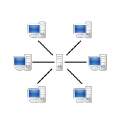
\includegraphics[width=\textwidth]{server-based-net.png}
        \caption{Server based network}
        \label{fig:server-based-net}
    \end{subfigure}\qquad
    \begin{subfigure}[h]{0.3\textwidth}
        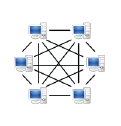
\includegraphics[width=\textwidth]{p2p-based-net.png}
        \caption{P2P based network}
        \label{fig:p2p-based-net}
    \end{subfigure}
    \caption{Tipologie di network}
    \label{fig:net}
\end{figure}\\\\
A differenza di una rete \textit{server based}, in una rete \textit{peer-to-peer} [\textbf{Figura~\ref{fig:p2p-based-net}}] (anche detta \textit{P2P}) non esiste la presenza di un server centrale che invia informazioni e tutti i dati vengono scambiati direttamente tra i nodi collegati alla rete. Ogni utente è quindi un \textit{client} ed un \textit{server} contemporaneamente.
Proprio per questa duplice funzione ogni dispositivo connesso viene detto \textit{nodo} della rete.\\
La sostanziale differenza tra le due tipologie di rete risiede nel fatto che mentre nel primo caso il \textit{server} contiene tutte le informazioni, nel secondo sono tutti e soli i \textit{client} a contenere i dati.\\
Ciò significa che nel primo caso il proprietario del \textit{server} può aggiungere, modificare o eliminare i dati che sono contenuti in esso, mentre nel secondo, anche se un nodo cancella o modifica i propri dati, gli altri nodi conterranno comunque tutte le informazioni originali. Da qui il termine distribuito.\\
\`E ora possible riprendere in mano la definizione originale: \textit{blockchain} è una tecnologia che permette di creare e gestire un grande archivio di informazioni, non contenute in un unico posto, ma del quale esiste una copia in ogni nodo connesso alla rete.

\subsection{Blockchain e Bitcoin}

\subsubsection{Ledger}
In letteratura è ritenuto più intuitivo usare \textit{Bitcoin} (\textit{BTC}) per esporre, tramite esempi semplificati, il funzionamento di una \textit{blockchain}.\\
Un \textit{Bitcoin} è una singola unità di valuta digitale che, proprio come l'\textit{Euro} non ha valore intrinseco, se non quello intenzionalmente attribuitogli grazie al consenso di scambio per l'acquisizione di beni o servizi.\\
%----------------------------------------------------------------------------------------
%	FIGURA 2
%----------------------------------------------------------------------------------------
\begin{wrapfigure}{r}{0.35\textwidth}
	\vspace{-31pt}
	\begin{center}
    	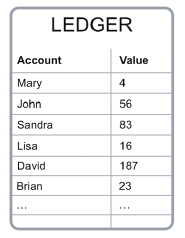
\includegraphics[width=0.37\textwidth]{ledger.png}
  	\end{center}
  	\vspace{-10pt}
  	\caption{Ledger}
  	\label{fig:ledger}
  	\vspace{-30pt}
\end{wrapfigure}
Per tenere traccia della quantità di \textit{Bitcoin} che ogni utente possiede si utilizza ciò che viene definito un \textit{Ledger} (libro mastro), che altro non è che un file in cui viene tenuta traccia di tutte le transazioni.
Il \textit{ledger} non è contenuto in un server centrale come ad esempio quello di una banca, ma ne esiste una copia in ogni nodo partecipante alla rete. In [\textbf{Figura~\ref{fig:ledger}}] è riportato, anche se in modo estremamente semplificato, un esempio di \textit{ledger}. 
Anche se nella realtà un ledger è molto diverso da quello in figura, nella pratica il disegno rappresenta fedelmente la funzione principale ricoperta da ogni copia del \textit{ledger} posseduta dai singoli nodi.
Nella colonna \textbf{Account} viene riportato il nome del proprietario dei \textit{Bitcoin}, mentre nella colonna \textbf{Value} è indicata la quantità posseduta da ognuno dei partecipanti.\\\\\\\\\\\\
Mettiamo caso che David voglia inviare cinque \textit{Bitcoin} a Sandra.
Per farlo è necessario che David mandi un messaggio sulla rete, il quale contiene la richiesta di transazione ed il numero di Bitcoin da lui posseduti.
Come informazione aggiuntiva viene inoltre trasmessa la quantità di \textit{Bitcoin} che possederà Sandra nel caso in cui la transazione avesse luogo. 
Il messaggio viene raggiunto dai nodi vicini a David i quali aggiornano i propri ledger con il risultato della possibile transazione (cioè David -5 \textit{BTC} e Sandra +5 \textit{BTC}) e rinviano il messaggio ai nodi a loro adiacenti. 
In questo modo il messaggio si espande per tutta la rete.
%----------------------------------------------------------------------------------------
%	FIGURA 3
%----------------------------------------------------------------------------------------
\begin{figure}[h]\hfill
    \centering
    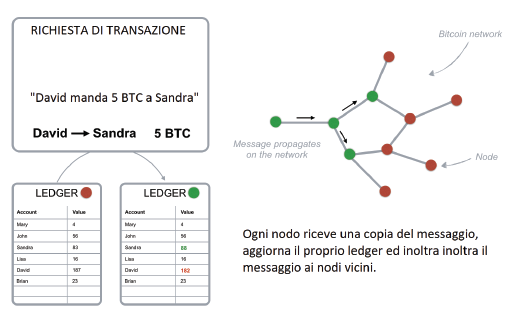
\includegraphics[width=\textwidth]{transaction.png}
    \caption{ Richiesta di transazione tra due nodi}
    \label{fig:transaction}
\end{figure}\\
Il fatto che il ledger sia mantenuto da tutti i nodi implica tre cose fondamentali, che stanno alla base del concetto della blockchain:
\begin{itemize}
\item  tutti sono a conoscenza di tutte le transazioni che avvengono sulla rete;
\item se la transazione non và a buon fine nessuno se ne prende la responsabilità in quanto non esiste un’entità centrale che si prenda carico dell’esito delle transazioni;
\item non esiste il bisogno di garanzie o fiducia in quanto la sicurezza è ottenuta tramite particolari funzioni matematiche estremamente sicure.
\end{itemize} 
\pagebreak

\subsubsection{Transazioni}
Perchè una transazione possa avere luogo è necessario ciò che viene definito un \textit{Wallet} (portafogli), ossia un software che permetta di depositare e scambiare scriptovaluta, tra cui \textit{Bitcoin}.
Poichè deve essere possibile solo ed esclusivamente al proprietario di un determinato \textit{Wallet} inviare i propri \textit{Bitcoin}, ogni \textit{Wallet} è protetto tramite una tecnica crittografica che usa una coppia di chiavi tra loro connesse.
Esse prendono il nome di chiave privata (\textit{private key}) e chiave pubblica (\textit{public key}).
%----------------------------------------------------------------------------------------
%	FIGURA 4
%----------------------------------------------------------------------------------------
\begin{figure}[h]\hfill
    \centering
    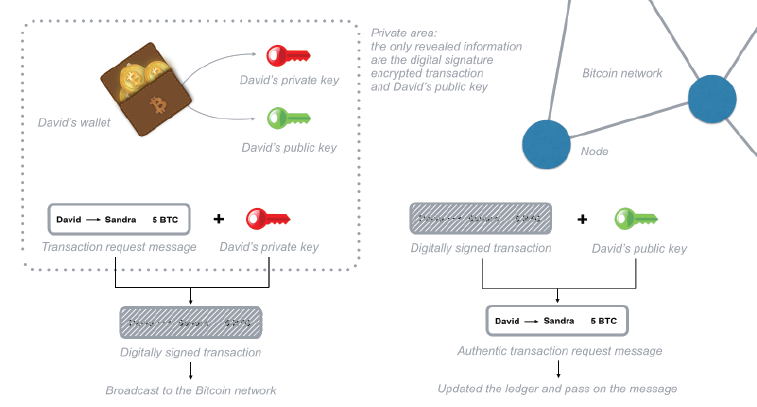
\includegraphics[width=\textwidth]{public-private-keys.png}
    \caption{Verifica della transazione tramite chiavi}
    \label{fig:pkey}
\end{figure}\\
Ogni messaggio in uscita da un singolo indirizzo viene criptato con una chiave privata il quale, una volta derivata la corrispondente chiave pubblica con cui è possibile identificare univocamente l'indirizzo di partenza (\textit{from}),deve poi essere validato dal nodo locale.
La validazione è necessaria per accertarsi che la transazione sia stata realmente messa sulla rete dal proprietario dell'account.
A questo punto solo i possessori della chiave pubblica associata potranno decifrare il messaggio.\\
Quando David vuole mandare 5 \textit{Bitcoin} a Sandra, deve inviare sulla rete il messaggio criptato con la sua chiave privata in modo che venga identificato come il possessore di un certo numero di \textit{Bitcoin} e sia di conseguenza l’unico a poter sbloccare il proprio \textit{Wallet}.
Tutti gli altri nodi validano la transazione, verificando tramite la chiave pubblica di David che la richiesta di inviare valuta sia effettivamente partita da lui.
In questo modo si ottiene la validazione della transazione.
In altre parole per poter inviare un \textit{Bitcoin} è necessario provare alla rete di essere i possessori dell'indirizzo da cui partono i \textit{Bitcoin}.\\
Nella rete inoltre non viene tenuto conto del bilancio dei singoli utenti, ma vengono semplecemente registrate le transazioni che avvengono.
La verifica di una transazione in questo modo si riduce semplicemente al controllo di tutte le transazioni passate, effettuate dall’utente che vuole inviare una certa somma di \textit{Bitcoin}.

\subsubsection{Blocchi}
Su una \textit{blockchain} le transazioni vengono ordinate tramite accorpamento con altre transazioni avvenute in un lasso di tempo definito.
In altre parole più transazioni vengono raggruppate insieme ed inserite dentro a quello che viene chiamato \textit{Block} (Blocco). 
Ogni \textit{block} contiene quindi un definito numero di transazioni ed un collegamento al nodo precedente. 
In questo modo si viene a creare una catena di blocchi molto simile ad una \textit{linked list}.
Da qui il nome \textit{blockchain} (catena di blocchi).
%----------------------------------------------------------------------------------------
%	FIGURA 5
%----------------------------------------------------------------------------------------
\begin{figure}[h]\hfill
    \centering
    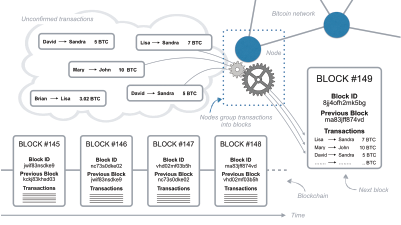
\includegraphics[width=\textwidth]{blocks.png}
    \caption{Rappresentazione di una blockchain}
    \label{fig:blocks}
\end{figure}\\
Le transazioni contenute nello stesso blocco sono considerate come avvenute nello stesso lasso temporale, mentre le transazioni che ancora non sono state raggruppate in un blocco sono considerate \textit{Unconfirmed}, cioè non ancora validate.\\ 
Ogni nodo della rete può raggruppare più transazioni e creare un blocco, suggerendo alla rete di inserirlo come prossimo blocco della catena. \\
Per essere effettivamente inserito nella rete un blocco deve contenere la soluzione ad un complesso problema matematico che, per essere risolto richiede una grossa potenza di calcolo, ed un pò di fortuna.
La risposta altro non è che un numero e l'unico modo per sapere quale sia il numero corretto da inserire consiste nel provarli tutti.
Il nodo che per primo risolve il problema acquisisce il diritto di inserire il prossimo blocco sulla catena e lo invia a tutti i nodi adiacenti.

\subsubsection{Mining}
A questo punto sorge spontaneo una domanda, ossia: "Se i Bitcoin posseduti da un account sono il risultato della somma di tutte le transazioni inviate e ricevute da quell'account, come è possibile ottenere altri \textit{Bitcoin}?"\\
La risposta a questa domanda é: "tramite il \textit{mining}".\\
Il \textit{mining} è l'attività svolta dai nodi definiti \textit{miners}, i quali, tramite la risoluzione di un complesso problema matematico, validano i blocchi, permettendo così a tutti i partecipanti alla rete di inviare e ricevere transazioni.\\
La validazione di un blocco nella pratica è una attività molto dispendiosa, sia in termini di energia elettrica che di consumo di banda.\\
Perchè la catena possa proseguire (cioè perchè possano essere effettuate nuove transazioni) è necessario che i blocchi siano inseriti nella catena e per farlo è necessario risolvere questo problema matematico.\\
Il modo escogitato per ripagare chi indovina il numero che valida il blocco (cioè svolge il lavoro di \textit{miner}) è una ricompensa in \textit{Bitcoin} da parte della rete. 
Questa ricompensa è ciò che incentiva le persone a provvedere al necessario lavoro computazionale per far continuare la catena e mantenere la rete utilizzabile. Senza i \textit{miners} i blocchi non potrebbero essere validati, la catena si fermerebbe e le transazioni non potrebbero più avere luogo.

\pagebreak
\subsection{Ethereum}

\subsubsection{Cos'é Ethereum}

Come \textit{Bitcoin}, \textit{Ethereum} è una \textit{public blockchain}.\\
Sebbene ci siano alcune significative differenze tecniche tra le due, la distinzione più importante da notare è che \textit{Bitcoin} ed \textit{Ethereum} differiscono sostanzialmente per scopo e capacità.\\
Il \textit{Bitcoin} è stato lanciato come valuta alternativa, o moneta digitale, ed offre una particolare applicazione della tecnologia \textit{blockchain}, ossia un sistema di pagamento elettronico.\\
\textit{Ethereum} invece viene principalmnte utilizzato per applicazioni decentralizzate tramite l'utilizzo degli \textit{Smart Contract}.\\
A differenza di \textit{Bitcoin}, \textit{Ethereum} utilizza due concetti di \textit{token}: il primo prende il nome di \textit{Ether} e corrisponde alla "moneta" effettivamente scambiata tra gli utenti della rete, il secondo viene invece utilizzato per pagare i \textit{miners}, i quali includono le transazioni nei blocchi, e prende il nome di \textit{gas}.

\subsubsection{Smart Contract}

Uno \textit{Smart Contract} è un programma che contiene un insieme di regole a cui le parti interessate accettano di aderire.\\
Nel caso in cui le regole definite all'interno di uno smart contract siano soddisfatte l'accordo tra le parti viene automaticamente applicato.\\
Il codice di uno \textit{Smart Contract} facilita, verifica e impone la negoziazione o l'esecuzione di un accordo o di una transazione e corrisponde alla forma più semplice di automazione decentralizzata.\\
Il successo di \textit{Ethereum} (e la più grande differenza con \textit{Bitcoin}) dipende proprio dal concetto di \textit{Smart Contract}. grazie a cui è possible programmare una serie definita di azioni che vengono attuate se e solo se le condizioni in esso contenute vengono soddisfatte.

%----------------------------------------------------------------------------------------
%	Sgame Pro
%----------------------------------------------------------------------------------------

\section{La piattaforma Sgame Pro}
%----------------------------------------------------------------------------------------
%	FIGURA 5
%----------------------------------------------------------------------------------------
\begin{figure}[h]\hfill
    \centering
    
\includegraphics[width=\textwidth]{sgamepro-logo.png}
    \label{fig:sgamepro}
\end{figure}
\textit{Sgame Pro} è un aggregatore di \textit{mobile games} di proprietà di \textit{Sgame SA}, con sede a Lugano, Svizzera.\\
In sviluppo dal 2016, Sgame Pro ha lanciato con successo la sua \textit{Alpha version} nel 2017, raggiungendo oltre 50.000 download senza nessuna spesa di marketing.\\
\textit{Sgame Pro} è interamente focalizzato sull'industria dei \textit{mobile games} e ha sviluppato due importanti innovazioni tecniche:
\begin{itemize}
	\item Consentire ai giocatori di essere remunerati con un nuovo utility token (\textit{SGM}) semplicemente giocando con il proprio cellulare ai titoli proposti;
	\item Aggregare il frammentato settore dei \textit{publisher}, indipendenti e non, in un'unica piattaforma di gioco \textit{one-stop-shop}.
\end{itemize}
 L'\textit{SGM} (token di tipo \textit{utility} basato sullo standard \textit{Ethereum ERC-20}) sarà l'unico modo per accedere ai servizi e beneficiare di tutte le funzinalità messe a disposizione degli utenti, oltre ad essere il metodo di pagamento unico per tutte le transazioni all'interno dell'ecosistema della piattaforma.\\
All'interno dell'applicazione i giocatori non solo avranno l'opportunità di trovare tutti gli ultimi titoli mobile resi disponibli, ma avranno anche l'opportunità di sfidare gli altri utenti sia in privato che tramite la funzionalità di \textit{Public Challenge}.\\
Quest'ultima innovazione è davvero dirompente dato che il 78\% del mercato dei giochi mobile è single player, mentre la maggior parte delle entrate derivano da giochi multiplayer.\\
Gli \textit{Influencers} di \textit{Sgame Pro} includono \textit{Pewdiepie}, \textit{Tweakbox} e molti altri, con oltre 80 milioni di seguaci altamente coinvolti e sparsi in tutto il mondo.\\ 



\bibliographystyle{abbrv}
\bibliography{thesis}

\end{document}
